%%  Copyright (C) 2016 Juan Manuel Torres Palma <j.m.torrespalma@gmail.com>
%%  This file is part of the SC-RSA program.
%%
%%  SC-RSA is free software: you can redistribute it and/or modify
%%  it under the terms of the GNU General Public License as published by
%%  the Free Software Foundation, either version 3 of the License, or
%%  (at your option) any later version.
%%
%%  SC-RSA is distributed in the hope that it will be useful,
%%  but WITHOUT ANY WARRANTY; without even the implied warranty of
%%  MERCHANTABILITY or FITNESS FOR A PARTICULAR PURPOSE.  See the
%%  GNU General Public License for more details.
%%
%%  You should have received a copy of the GNU General Public License
%%  along with SC-RSA.  If not, see <http://www.gnu.org/licenses/>.  */

\documentclass[pdf]{beamer}
\mode<presentation>{}

\usepackage{xeCJK}
\usepackage{wrapfig}
\setCJKmainfont{VL Gothic}
\usepackage{amssymb}
\usepackage{pifont}
\usetheme{Szeged}
\usecolortheme{beaver}
\useinnertheme{circles}
\useoutertheme{infolines}
\usepackage{multicol}

\usepackage{algpseudocode}

%% preamble
\title[SC-RSA]{Asymmetric Cryptography: RSA}
\author[Juan Manuel Torres Palma]{Juan Manuel Torres Palma}
\institute[UGR]{Universidad de Granada}

%% Used to show TOC before each section beginning
\AtBeginSection[]
{
\begin{frame}{Table of contents}
\tableofcontents[currentsection]
\end{frame}
}

\begin{document}

%% title frame
\begin{frame}
\titlepage
\end{frame}

\begin{frame}{Table of contents}
\tableofcontents
\end{frame}

%%
\section{Cryptography}
\begin{frame}{Cryptography}
	\textbf{Cryptography} is a science that uses mathematics in a
	way that makes data impossible to read (Ciphertext) for those
	that are not in possesion of a key that allows them to read it.
	\vspace{1cm}
	\begin{itemize}
	\item \textbf{Symmetric.} The same key is used to encrypt and
	decrypt.
	\item \textbf{Asymmetric.} Different keys are used to encrypt and
	decrypt.
	\end{itemize}
\end{frame}

\section{Asymmetric Cryptography}
\begin{frame}{Asymmetric Cryptography}
	\begin{columns}
	\column{0.4\linewidth}
		\begin{itemize}
		\item Bob: Uses Alice's \textbf{public key} to encrypt.
		\item Alice: Uses her \textbf{private key} to decrypt.
		\item Key is a number or set of numbers that applied to the
		message, makes it impossible to read.
		\item The bigger the key, the harder to break.
		\end{itemize}
	\column{0.6\linewidth}
		\centering
		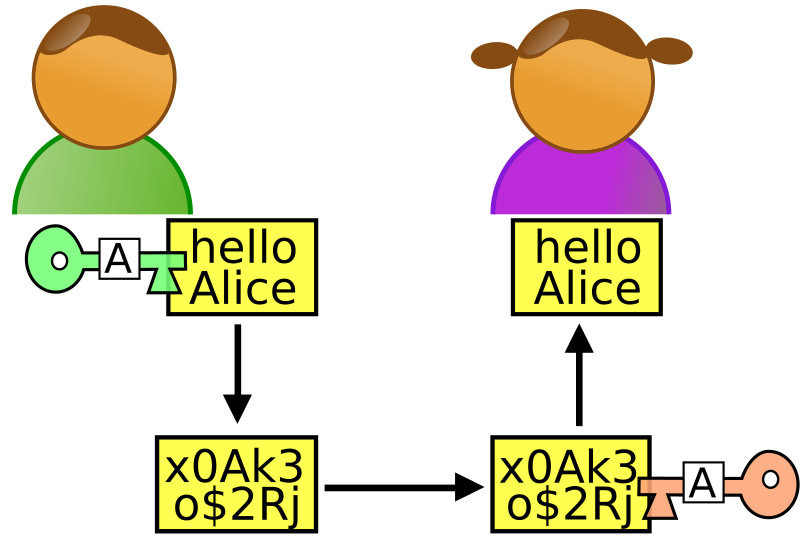
\includegraphics[scale=0.2]{img/serveimage.png}
	\end{columns}
\end{frame}

\section{Practical example: RSA-32}
\subsection{RSA-32: Key generation}
\begin{frame}{RSA-32\footnote{Used for simplicity, RSA-1024 recommended.}: Key generation}
	\textbf{Key generation algorithm}
	\begin{footnotesize}
	\begin{columns}[t]
	\column{0.5\linewidth}
	\begin{algorithmic}
		\State $e\gets 3$
		\Repeat
			\State $p\gets genprime()$
		\Until $(p\ mod\ e) \neq 1$
		\Repeat
			\State $q\gets genprime()$
		\Until $(q\ mod\ e) \neq 1$
	\end{algorithmic}
	\column{0.5\linewidth}
	\begin{algorithmic}
		\State $N\gets p\times q$
		\State $L\gets (p-1)(q-1)$
		\State $d\gets modinv(e,\ L)$
		\State \Return $(N,\ e,\ d)$
	\end{algorithmic}
	\end{columns}
	\end{footnotesize}
	\vspace{0.2cm}
	\begin{block}{Generating keys}
		\centering
		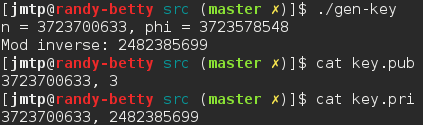
\includegraphics[scale=0.4]{img/gen-key.png}
	\end{block}
\end{frame}

\subsection{RSA-32: Encrypt}
\begin{frame}{RSA-32: Encrypt}
	\textbf{Encryption algorithm}
	\begin{algorithmic}
		\State $(n,\ e)\gets readkey(pub)$
		\State $c\gets (m^e\ mod\ n)$
		\State \Return $c$
	\end{algorithmic}
	\vspace{1cm}
	\begin{block}{Encypting a message}
		\centering
		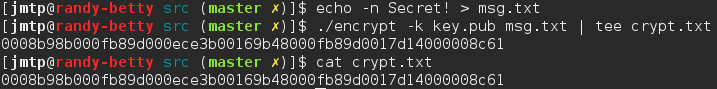
\includegraphics[scale=0.4]{img/encrypt.png}
	\end{block}
\end{frame}

\subsection{RSA-32: Decrypt}
\begin{frame}{RSA-32: Decrypt}
	\textbf{Decryption algorithm}
	\begin{algorithmic}
		\State $(n,\ d)\gets readkey(pri)$
		\State $m\gets (c^d\ mod\ n)$
		\State \Return $m$
	\end{algorithmic}
	\vspace{1cm}

	\begin{block}{Decrypting a message}
		\centering
		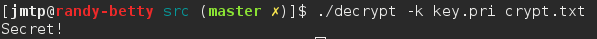
\includegraphics[scale=0.4]{img/decrypt.png}
	\end{block}
\end{frame}

\section{References}
\begin{frame}{References}
	\begin{itemize}
		\item \textbf{RSA algorithm theory explained:}
		\href{http://www.di-mgt.com.au/rsa_alg.html}
		{\textcolor{cyan}{Link.}}
		\item \textbf{SC-RSA implementation:}
		\href{https://github.com/jmtorrespalma/sc-rsa}
		{\textcolor{cyan}{GitHub.}}
	\end{itemize}

\end{frame}

\end{document}
